\documentclass[ngerman]{tudscrreprt}
\usepackage{selinput}
\SelectInputMappings{adieresis={ä},germandbls={ß}}
\usepackage[T1]{fontenc}
\usepackage{babel} 
\usepackage{isodate}
\usepackage{amssymb}
\usepackage{amsmath}
\usepackage{float} % lädt das Paket zur Verwendung von zusätzlichen Positionsbefehlen
\usepackage{wrapfig}    % vor der Zeile \begin{document} einfügen
\usepackage{picinpar}     % vor der Zeile \begin{document} einfügen 
\usepackage{float} % lädt das Paket zur Verwendung von zusätzlichen Positionsbefehlen
%----------------------
\usepackage{listings}
\usepackage{graphicx} 
\usepackage{color} 
\usepackage{transparent} 
\usepackage{relsize}
\usepackage{ulem}

%----------
\usepackage{hyperref}
%----------
\definecolor{dkgreen}{rgb}{0,0.6,0}
\definecolor{gray}{rgb}{0.5,0.5,0.5}
\definecolor{mauve}{rgb}{0.58,0,0.82}

\lstset{frame=tb,
  language=Java,
  aboveskip=3mm,
  belowskip=3mm,
  showstringspaces=false,
  columns=flexible,
  basicstyle={\small\ttfamily},
  numbers=none,
  numberstyle=\tiny\color{gray},
  keywordstyle=\color{blue},
  commentstyle=\color{dkgreen},
  stringstyle=\color{mauve},
  breaklines=true,
  breakatwhitespace=true
  tabsize=3
}
%----------------------


\begin{document}
\faculty{Fakultät Elektrotechnik und Informationstechnik} \department{} \institute{Institut für Regelungs - und Steuerungstheorie} \chair{Prof. Dr.-Ing. habil. Dipl. Math. Klaus Röbenack} \title{Prozessidentifikation 1{\footnote{Mitschrift von Bolor Khuu}}
}

% \thesis{diss}
% \degree[Dr.-Ing.]{Doktor-Ingenieur}
\author{Prof. Dr.-Ing. habil. Dipl. Math. Klaus Röbenack}
% \dateofbirth{2.1.1990}
% \placeofbirth{Dresden}
% \date{20.08.2014}
% \defensedate{20.10.2014}
% \referee{Dagobert Duck \and Mac Moneysac}
\maketitle
\tableofcontents
\newpage
\chapter{Einführung}
	\section{Aufgaben und Ziele der Prozessanalyse}
	\begin{itemize}
	\item System:\\Abgegrenzte Anordnung von aufeinander einwirkende Gebilden
	\item Prozess:\\Umformung oder Transfort von Materie Energie bzw. Information
	\item Prozess und Systemanalyse:\\Gewinnung mathematischer Modelle von Prozessen bzw. Systemen
	\end{itemize}
	Nutzung von Modellen:
	\begin{itemize}
	\item Vorhersage (Simulation)
	\item Verbessern des Verhaltens des Systems (Optimierung Regelung)
	\end{itemize}


	Prozessanalyse $\leftrightarrow$ Signalanalyse $\leftrightarrow$ Systemanalyse\\

	Systemanalyse:
	\begin{itemize}
	\item Modell (Aufgabestellung)
	\item statische bzw. stationäre Modell
	\item dynamische Modell 
	\begin{enumerate}
		\item Modelle mit konzentrierten Parameter (gewöhnliche DGL) ODE
		\item Modelle mit verteilten Parameter\\ (Partielle DGL) Wärmeleitung, Maxwellsche Partielle DGL
	\end{enumerate}

	Beispiel:\\

	\subitem -Schalter 
	\begin{figure}[H] 
		\centering 
		\def\svgwidth{100pt} 
		%\input{Zeichnung.pdf_tex} 
		\input{prozessid00.pdf_tex} 
		%\caption{Diodenkennlinie} 
	\end{figure} 

		% \begin{figure}[htbp]
		% 		\def\svgwidth{100pt} 
		% 		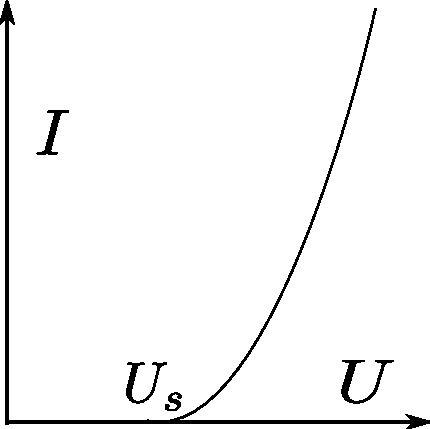
\includegraphics[width=7.5cm]{prozessid00.pdf}
		% \end{figure}
	\subitem -statischer Modell $I = I_s (e^{\frac{U}{mU_T} } - 1).$
	\begin{figure}[H] 
		\centering 
		\def\svgwidth{100pt} 
		%\input{Zeichnung.pdf_tex} 
		\input{prozessid01.pdf_tex} 
	\end{figure} 

	\subitem -dynamischer Modell $\rightarrow$(Kapazitätsdiode)
	
	\item Verwendungszweck bestimmt 
			\begin{itemize}
			\item{Darstellungsform}
			\begin{enumerate}
				\item nicht parametrisch (graphisch oder tabelarisch). Darstellung von Systemcharakteristiken
				\item parametrisch (Symbolische Ausdrücke mit Struktur z.B Polynom gebrochen rationale Funktion)
			\end{enumerate}
			\end{itemize}
			\begin{itemize}
				\item Darstellungsbereich
	 		\begin{enumerate}
				\item Amplitudenbereich (z.B: statische Kennlinie)
				\item Zeitbereich (z.B: Gewichtfunktion, Sprungantwort)
				\item Spektralbereich (z.B: Übertragungsfunktion $G(s)$ Frequenzgang)
			\end{enumerate}

			\end{itemize}	
		
	\item Nutzung von A-priori-Information \\
		über wichtige Modelleigenschaften \\
		z.B: linear/nicht linear
	\end{itemize}

	\section{Allgemein Strategien}

	Modellvereinfachung dynamischer Modell bei der theoretischen Prozessanalyse \\

	Modelle mit verteilten Parameter (partielle DGL) Diskretisierung (örtlich) Modellanalyse\\
	\begin{equation*} 
	\downarrow
	\end{equation*}
\\
	Modelle mit konzentrierten Parameter (gewöhnliche DGL.) Linearisierung (im Arbeitspunkt).\\
	Lineares Modell, lineare DGL. Ordnung $n$ Ordnungsreduktion\\
	\begin{equation*} 
	\downarrow
	\end{equation*}
	Lineares Modell , lineare DGL. Ordnung $1<n$. 

\begin{itemize}
\item Aktive bzw. passive Experimentation
	\begin{itemize}
	\item
	\begin{itemize}
			\item Merkblatt
		\end{itemize}
	\item Aktive Experimentation (z.B Sprung)
		\begin{itemize}
			\item Testsignal Sinusschwingung, Rausch-Signal
		\end{itemize}
\item Passive Experimentation Messung im laufenden Betrieb
\item Aktive passive Experimentation
	\end{itemize}
\end{itemize}
\newpage
	\section{Modellvorstellung zu Prozessen}
	\begin{enumerate}
	\item Prozesse in MIMO-Struktur (vektorielle Einflußgrößen Vereinfachung prüfen)
	\subitem MIMO-MISO.
	\subitem MISO-SISO.
	\begin{itemize}
	\item Bemerkung: Teimodelle müssen unbedingt mit Teilaufgaben übereinstimmen.
	\end{itemize}
	\item Präzisierung der Modellvorstellung \\

		\begin{figure}[H] 
		\centering 
		\def\svgwidth{300pt} 
		%\input{Zeichnung.pdf_tex} 
		\input{bild00.pdf_tex} 
		\end{figure} 

		Modellvorstellung der Einstellgrößen $\varepsilon, z_1 \dots z_4 \dots w.$
		\begin{itemize}
		\item Realisierung von Zufallsvektoren $\varepsilon, z_1 \dots z_4 \dots w.$
		\item oder: Realisierung von Zufallsprozessen $\varepsilon(t), z_1(t).$ 
		\item oder: (einfach) unbekannte Werte
		\end{itemize}
	\item Vereinfachung prüfen
		\begin{enumerate}
		\item Signifikant von Einstellfehlern von $u$, ggf $\varepsilon=0$
		\item Signifikant von Messfehler von $u,V$, ggf $z_1 =0 \quad z_2 = 0$
		\item Abhängigkeiten der Signale
		\item Prozessstörung $w$ werden als auf $x^0, y^0$ Transfonierte Störung behandelt.

		\begin{figure}[H] 
		\centering 
		\def\svgwidth{200pt} 
		%\input{Zeichnung.pdf_tex} 
		\input{bild01.pdf_tex} 
		\end{figure} 

		\item Signifikant der Einflußgrößen
		$\rightarrow$ Reduktion der Dimension
		\item Dekomposition (Zerlegung z.B in MISO-SISO)
		\end{enumerate}

	\end{enumerate}


\chapter{Problemformulierung für statische Modelle}
	\section{Einf\"uhrungsbeispiel}
	Modellansatz: $y = a+ b\cdot u \leftrightarrow 0=y - a - b\cdot u$\\
	Fragestellung: 
	\begin{itemize}
	\item kann man ähnliche explizite Schätzregeln auch für mehrvariable bzw. nichtlineare Modelle erhalten?
	\item Für welche Klassen nichtlinearer Modelle sind ähnlich Schätzregeln leicht zu gewinnen?
	\item Welche Fehlermaße sind zu verwenden?
	\end{itemize}
	\section{Unterteilung statischer Modelle}
	$U, Y \dots$ Vektorräume \\ 
	Eine Abb. $f: U \to Y $ heißt linear, wenn für alle Vektoren $u, v \in U$ sind alle Skalare $\alpha, \beta$ gilt. \\ 
	\begin{align*}
	f(\alpha v) &= \alpha f(v) \qquad \text{Homogenität}\\ 
	f(u+v) &= f(u) + f(v) \qquad \text{(Additivität)}
	\end{align*}
	Gleichbedeutend (Superposititionsprinzip)\\ 
	\begin{align*}
	f(\alpha u + \beta v) = \alpha f(u) + \beta f(v)
	\end{align*}
	Bsp: $U = V = \mathrm{R} , \qquad f(u) = a + b u $ mit $a,b \in \mathrm{R}$
	\section{Linearit\"at (Allgemein)}
		Seien $U$ und $Y$ zwei Verktorräume. Ein Abbildung $f: U \rightarrow Y $ heißt linear, wenn für alle Vektoren $u, v \in U$ und alle Skalare $\alpha , \beta $ die Bedingungen
			\begin{enumerate}
			\item $f(\alpha \cdot v) = \alpha \cdot f(v)$ Homogenität
			\item $f(u + v) = f(u) + f(v)$ Additivität erfüllt sind. Diese zwei Bedingungen sind gleichbedeutend mit:
			\item $f(\alpha \cdot u + \beta \cdot v) = \alpha f(u) + \beta f(v)$ 
			\end{enumerate}

	\section{Linearit\"at und Parameterlinearit\"at}
		Wir betrachen statische, parametrische Modelle der Form $\underline{y} = f(\underline{u}, \underline{a})$ und den zusätzlichen Parametervektor $ \underline{a}.$
	\begin{itemize}
	\item Definition:\\Die Funktion $f$ heißt \textit{linear}, wenn sie bezüglich $\underline{u}$ linear ist für alle $\underline{a}.$\\
	Die Funktion $f$ heißt \textit{parameterlinear}, wenn sie bezüglich des Parametervektors $\underline{a}$ linear ist für alle $\underline{u}.$ \\ 
	\item Bsp: 1. Polynome in $u (u, y, )$ skalar: \\ 
	\begin{align*}
	y = f(u,a) &= a_0 + a_1 u + a_2 u^2 + \dots + a_n u^n \\
	&= (1, u, u^2, \dots, u^n)\begin{pmatrix}
	a_0\\ a_1\\ a_2\\ \vdots\\ a_n
	\end{pmatrix}
	\end{align*}
	nichtlinear aber parameternichtlinear.
	\item Bsp: 2. Polynome in mehreren Variablen, \\ 
	z. B. $ u = \begin{pmatrix} u_1\\ u_2 \end{pmatrix}$
	\begin{align*}
	y = f(u,a) &= a_1 u_1^2 + a_2u_2^2 + a_3 u_1 u_2\\ 
	&= (u_1^2, u_2^2, u_1 u_2)\begin{pmatrix} a_1 \\ a_2\\ a_3 \end{pmatrix}
	\end{align*} 
	nichtlinear, aber parameterlinear.
	\item Bsp: 3. Strom-Spannungs-Kennlinie eine Flächendiode:
	\begin{align*}
	i = I_s (e^{\frac{u}{m U_T}} - 1)\\ 
	I_S \dots \qquad \text{Sättigungsstrom}\\ 
	U_T \dots \qquad \text{Temperaturspannung}\\ 
	m \dots \qquad \text{Koeff } (m = 1 \dots 2)\\ 
	a = \begin{pmatrix} a_1\\ a_2 \end{pmatrix} = \begin{pmatrix} I_S \\ mU_T\end{pmatrix}
	\end{align*}
	\item Fazit:\\Parameterlineare statische SISO- und MISO Modelle lassen sich als Skalarprodukte einer Funktion $\rho: \mathbb{R}^m \rightarrow \mathbb{R}^n $ (SISO$:m=1$) mit dem Parametervektor $\underline{a} \in \mathbb{R}^n$ darstellen:\\$y=\rho^T(\underline{u})\underline{a} = \underline{a}^T \rho(\underline{u})$
	\end{itemize}
	\section{Problemformulierung}
		\subsection{Fehlermodelle}
		Ausgangsmodell für den Fehler: $\varepsilon = y - \tilde{y}$ 
		\begin{itemize}
		\item System: $y = f(u,a) + z$
		\item Modell: $\tilde{y} = f(u,\tilde{a})$
		\item Gütekriterium: Bei MIMO-Systemen bzw. bei mehreren Messwerten ist $\varepsilon$ vektorwertig. Es bietet sich die Verwendung eines Gütekriteriums an. Die Minimierung bezüglich des Parameters $a$ liefert den \textit{optimalen} Parameter $\tilde{a}$

		\begin{itemize}
		\item ungestörter oder schwach gestörter Fall $z\approx0$ Approximationsproblem
		\item gestörter Fall $\rightarrow$ Parameterschätzproblem
		\end{itemize}
		\end{itemize}
		\subsection{G\"utekriterium: Normen}
		\begin{itemize}
		\item Eigenschaften: 
		\begin{enumerate}
		\item $\parallel x \parallel = 0 \leftrightarrow x= 0 \quad \forall x$
		\item $\parallel \alpha x \parallel = |\alpha| |x| \quad \forall \alpha, x$
		\item $\parallel x + y \parallel \leq \parallel x \parallel + \parallel y \parallel \quad \forall x,y$ 
		\end{enumerate}
		\item Merke:\\
		Der Normoperator bildet den Vektor auf eine reelle Zahl ab. Aus den Eigenschaften folgt, dass eine Norm nur nichtnegative Werte annehmen kann \\
		$ 0 = \| 0 \| = \| x-x \| + \| -x \| = \| x \| + \| x \| = 2 \| x \| \Rightarrow \| x \| \geq 0$\\
		Beispiele für Normen:\\

		$\underline{x} \in \mathbb{R}^m , x= 
		\begin{pmatrix}
		&x_1& \\
		&\vdots&\\
		&x_m& 
		\end{pmatrix}
		$
		\end{itemize}
		\begin{itemize}
		\item Spaltensummen-Norm (1-Norm):
		$\|\underline{x}\|_1 = |x_i| + \dots +|x_m|$
		\\ Matlab: $norm(x,1)$\\
		\item Euklidische Norm (2-Norm):$\qquad \|x\|_2 = \sqrt[2]{|x_1|^2 + \dots + |x_m|^2} = \sqrt{x^T x}$\\
		\\ Matlab: $norm(x)$ oder $norm(x,2)$\\
		\item p-Norm:$\qquad \|\underline{x}\|_p = \sqrt[p]{|x_1|^p + \dots + |x_m|^p}$\\
		\item Maximum-Norm oder Tschebyschew-Norm:
		$\|\underline{x}\|_\infty = max{|x_1| , \dots , |x_m|}$\\
		\item Wikipedia: Die Maximumnorm ist \textit{formal keine $p-$Norm, kann aber als Grenzfall für $p\rightarrow \infty$ aufgefasst werden.}
		\item Verwendung von Normen bei Approximationsproblemen:
		\end{itemize}
		\begin{itemize}
		\item 2-Norm $\Rightarrow$ direkte (explizite) Schätzregeln möglich.
		\item andere Normen $\Rightarrow$ i.d.R nur numerisch mit Optimierungssoftware möglich.

		\item Bsp: \begin{align*}
		x = \begin{pmatrix}
		1\\ 2\\ 3
		\end{pmatrix}, \|x\|_1 = 6, \| x\|_2 \approx 3.74, \|x\|_{\infty} = 3
		\end{align*}\\ 
		Für quadratische integrierbare Fkt. $u:[0, \infty) \to \mathrm{R}$ ist \begin{align*}
		\|u\|_2 = \sqrt{\int_0^{\infty} [u(t)]^2 dt}
		\end{align*}
		eine Norm.\\
		Verwendung von Normen bei Approximationsproblemen \begin{itemize}
		\item 2 -Norm $\to$ direkte Schätzregel möglich
		\item andere Norm $\to$ in der Regel nur numerisch
		\end{itemize}
		\end{itemize}
\subsection{Abstand zwischen Vektoren: Metrik}
Mit \begin{align*}d(x,y) = \|x - y\| , \qquad x,y \in V \end{align*}
wird eine Metrik $d$ auf $V$ definit.\\ 
Eigenschaften (Metrik als Abstand):
\begin{enumerate}
\item $d(x,y) = 0 \leftrightarrow x=y$
\item $d(x,y) = d(y,x)$
\item Dreiecksgleichung:\begin{align*}
d(x,z) \le d(x,y) + d(y,z)
\end{align*}
\end{enumerate}
\chapter{Methode der kleinsten Fehlerquadrate}
	\section{Basisalgorithmus}

	Gütekriterium mit $\varepsilon_i = y_i - f(u_i,a), \qquad i = 1, \dots, N $ (Messwerte)
	\begin{itemize}
	\item ungewichtete MKQ:
	$q(\underline\varepsilon) = \sum\limits_{i=1}^N \varepsilon_i^2 = \underline\varepsilon^T \underline\varepsilon = \|\underline\varepsilon\|_2^2$
	\item gewichtete MKQ: statt einzelne Abweichungen $\varepsilon_i$ betrachte man gewichtete Abweichungen $w,\varepsilon$ mit Gewichten $w_i$ für $i=1 \dots N.$\\
	$q(\underline\varepsilon) = \sum\limits_{i=1}^{N} w_i^2 \varepsilon_i^2 = \underline\varepsilon^T W^T W \underline\varepsilon = \|W \underline\varepsilon \|_2^2$\\
	mit $w= diag(w_1 \dots w_N)= 
	\begin{pmatrix}
	w&\dots&0 \\
	\vdots&\ddots&\vdots\\
	0&\dots&w_N
	\end{pmatrix}
	\in \mathbb{R}^{N\times N}
	$ \\
	\item MKQ für parameterlineare Modelle:
	\begin{itemize} \item Modell: $y= f(u,a) = \varphi^T(u)a.$\\
	Für alle Messungen $(u_i,y_i)$ soll gelten. $y_i\approx \varphi^T(u_i)\underline a \quad$ für $\quad i=1 \dots N$\\
	Erfassung aller $N$ Messungen\\
\\	$
	\underbrace{\begin{pmatrix}
	&y_1&\\
	&\vdots&\\
	&y_N&
	\end{pmatrix}}_{\underline y \in \mathbb{R}^N}
	=
	\underbrace{
		\begin{pmatrix}
	&\varphi^T(u_1)&\\
	&\vdots&\\
	&\varphi^T(u_N)&
	\end{pmatrix}
	}_{\phi \in \mathbb{R}^{N\times n}}
	\cdot
	\underbrace{	\begin{pmatrix}
	&a_1&\\
	&\vdots&\\
	&a_N&
	\end{pmatrix}
}_{\underline a \in \mathbb{R}^n}
+
\underbrace{	
\begin{pmatrix}
&\varepsilon_1&\\
&\vdots&\\
&\varepsilon_N&
\end{pmatrix}
}_{\underline{\varepsilon} \in \mathbb{R}^N}
	$ 
\end{itemize}
\item In der Regel: $N\geq n$ (Mehr Messwerte als Parameter) \\Gleichungssystem ist überbestimmt $\rightarrow$ In der Regel NICHT lösbar.
\begin{itemize}
\item Ausweg:\\ Minimale Fehler $\underline{\varepsilon}$ zwischen linker und rechter Seite des Gleichungssystem:($\star$).\\
$ 
\|\varepsilon\|_2 = \|y-\phi \underline{a}\|_2 = d(y, \phi \underline{a})\quad\text{ungewichtete MKQ}\\
\|w\underline{\varepsilon}\|_2 = \|w(y-\phi\underline{a})\|_2 \quad \text{gewichtete MKQ}
$ 
\begin{figure}[H] 
		\centering 
		\def\svgwidth{200pt} 
		\input{bild02.pdf_tex} 
\end{figure} 
Günstig $\| \cdot\|_2 \rightarrow min \leftrightarrow \|\cdot\|_2^2 \rightarrow min$
\\
\item \text{Gütefunktional:}\\
$ 
\begin{matrix}
 q= \|\underline{\varepsilon}\|_2^2&=& \underline{\varepsilon}^T \cdot \underline{\varepsilon}\\
 &\underbrace{=}_{\star}& (y-\phi \underline{a})^T(y-\phi \underline{a})\\
 & = & y^Ty - y^T \phi a - (\phi\underline{a})^T\cdot y + (\phi a)^T \phi a\\
 & = & y^T \cdot y - 2 y^T \phi \underline{a} + \underline{a}^T \phi^T \phi \cdot a
\end{matrix}
$ 
\end{itemize}
\item Gesucht: Gradient $ \frac{\partial{q} }{\partial{\underline{a}} } = \left( \frac{\partial{q}}{\partial{a_1}} \cdots \frac{\partial{q}}{\partial{a_n}} \right)  $
\\
\item Errinerung
\begin{itemize}
\item Aquadratisch:$ \frac{\partial}{\partial{x} }\cdot(x^T A x) = x^T (A + A^T)\\
$ 
\item \text{Asymmetrisch:} $\frac{\partial}{\partial{x}} (x^TAx)= 2 x^T A. $\\
d.h \begin{equation*} A= A^T\end{equation*}
\item Abweichung des Gütefunktionals nach dem Parametervektor $\underline{a}$ 
\begin{equation*}
\frac{\partial{q}}{\partial{a}} = -2 y^T \phi + 2 a^T \phi^T \phi
\end{equation*}
\item Notwendige Bedingung für lokale Extremum.
\begin{equation*}
\quad0^T =\frac{\partial{q}}{\partial{\underline{a}}} = -2y^T \phi + 2\underline{a}^T \cdot \phi^T \phi.\\
y^T \phi = \underline{a}^T \cdot \phi^T \cdot \phi,\qquad \phi^T y = \phi^T \phi a
\end{equation*}
\item System der Normalengleichung.\\
\item Lösung der Normalengleichungen falls $\phi^T \phi$ invertierbar. \\
\begin{equation*}
\hat{\underline{a}} = (\phi^T\phi)^{-1} \phi^T y
\end{equation*}
\end{itemize}
\item Zusammenfassung:\\
Nicht lösbares lineares Gleichungssystem. $y=\phi a.$\\
$
\begin{matrix}
\text{Minimierung des Fehlers} & \mathlarger{\mathlarger{\downarrow}}& \text{Gauß-Transformation} \\
					    & &				\text{Multiplikation}\\
		\|y-\phi \underline{a}\|_2^2 && \text{linkst mit } \phi^T 
\end{matrix}
$
\\
Normalengleichungen: $ \phi^T y = \phi^T \phi \underline{a}$\\
Geometrische Interpretation\\

$
\begin{matrix}
<\phi \underline{a}, \underline{\varepsilon} > = (\phi, \underline{a})^T\underline{ \varepsilon }& = &\underline{a}^T \phi^T (y-\phi \underline{a})\\
&=& a^T (\phi^T y - \phi^T \phi a) = 0 \\
&=& 0 \text{ für } a= \hat{a}
\end{matrix}
$\\ Lösung der Normalengleichung\\

$\rightarrow \underline{\varepsilon}$ stet senkrecht auf $\phi a,$\\
$\rightarrow \text{ von } y \text{ wird orthogonal auf die Ebene (KVR) projeziert} $
\\
\item Gewichtete MKQ:\\
Statt $\| y-\phi \underline{a} \|_2^2 \text{ wird }\quad
	   \|w(y-\phi a)\|_2^2 \text{ minimiert }
$\\
Substituation: $\tilde{y} = w \cdot y , \quad \tilde{\phi} = w \cdot \phi$
\begin{itemize}
\item Lösung der ungewichtete MKQ für $\|\tilde{y} - \tilde{\phi}\underline{a}\|_2^2$\\
\item Lösung: $\hat{\underline{a}} = (\tilde{\phi}^T \tilde{\phi})^{-1} \phi^T w^T w y$
\item Beispiel (ungewichtete MKQ) 
\item Meßwerte:
\item Ansatz:  $ y= a_0 + a_1 u + a_2 u^2 = \underbrace{(1 \quad u\quad u^2)}_{\phi^T(u)} \cdot
\underbrace{
	\begin{pmatrix}
&a_0&\\
&a_1&\\
&a_2&\
\end{pmatrix}
}_{\underline{a} \in \mathbb{R}^3} \quad n=3
$\\
$
\phi = 
\begin{pmatrix}
&\phi^T(u_1)&\\
&\vdots&\\
&\phi^T(u_5)& 
\end{pmatrix} = 
\begin{pmatrix}
1&0&0\\
1&1&1\\
1&2&4\\
1&4&16\\
1&5&25
\end{pmatrix} \in \mathbb{R}^{5\times 3} \quad \text{Meßvektor:} y=
\begin{pmatrix}
&12&\\
&4&\\
&1&\\
&5&\\
&13&
\end{pmatrix}
$ 
\\
\item System der Normalengleichung\\
$
\begin{pmatrix}
&35&\\
&91&\\
&413&
\end{pmatrix}
= 
\begin{pmatrix}
5&12&46\\
12&46&198\\
46&198&898
\end{pmatrix} \cdot \hat{\underline{a}} \qquad 
\phi^Ty \in \mathbb{R}^3 \quad \phi^T\phi \\
$ 
\item Parametervektor:
$
\hat{\underline{a}} = 
\begin{pmatrix}
&\hat{a}_0&\\
&\hat{a}_1&\\
&\hat{a}_2&
\end{pmatrix} = (\phi^T \quad \phi)^{-1} \phi^T y \approx 
\begin{pmatrix}
&11.86&\\
&-9.43&\\
&1.93&
\end{pmatrix}.
$
\end{itemize}
\end{itemize}
\section{Lösungsansätze für unbestimmte lineare Gleichungssysteme}%$ 
\section{Erinnerung: Lösbarkeit linearer Gleichungssystem.}%{Sinngulärwertzerlegung}
\label{Sec:Loesbarkeit.lin.Gleichungssystem}
\begin{itemize}
\item Lineares Gleichungssystem: \begin{equation*}Ax=b.\quad \tag{L} \end{equation*}\\
mit $A \in \mathbb{R}^{m\times n}, \quad b \in \mathbb{R}^m \quad x\in \mathbb{R}^n$\\
\item Lösbarkeit: Das Gleichungssystem(L) ist genau dann lösbar, wenn \\
rang $A = $rang$(A,b)$.\\ 

\item Interpretation: Der Vektor $b$ kann als linearkombination der Spalten \\$\underline{a}_1 \dots \underline{a}_n \in \mathbb{R}^m \quad \text{von } A=(\underline{a}_1 | \dots | \underline{a}_n). \text{  dargestellt werden.  } \\ Ax=b \leftrightarrow x_1, \underline{a}_1 + \dots + x_n \underline{a}_n = b.$ \\
Köffizienten der Linearkombination sind die Köffizienten der Lösung $x$.\\

\item Eindeutigkeit(unität): Gleichungssystem(L). in Lösbar. mit $r=rang A$ dann 
\begin{enumerate}
\item $r=n:$ Lösung ist eindeutig. d.h. Lösungsmenge ist ein einzelner Punkt $x\in \mathbb{R}^n$
\item $r<n:$ Lösung ist nicht eindeutig, Lösungsmenge ist eine $(n-r)$ - dim. lin. Mannigfestigkeit im $\mathbb{R}^n$ 
\end{enumerate}
\end{itemize}
\section{Rangbestimmung und Singul\"arzerlegung}
Sei $A \in \mathbb{R}^{m\times n}$ mit $r=rank A.$ .Dann gibt es orthogonale Matrizen $U \in \mathbb{R}^{m\times m}$ und $V \in \mathbb{R}^{n\times n}$ sowie eine Diagonalmatrix 
$ 
\begin{pmatrix}
\sigma_1&         &        &   &\\
        &\sigma_2 &        &   &0_{r\times (n-r)}\\
        &         & \ddots &   &\\
        &         &        &\sigma_r&\\
&&0_{(m-r)\times r }& & 0_{(m-r)\times (n-r)}
 
\end{pmatrix}
$
\\
derart ,dass gilt $ A = U \cdot S \cdot V^T$ \\
Die Zahlen
$\quad \sigma_1 \geq \sigma_2 \geq \dots \geq \sigma_r > \sigma_{r+1} = \dots= \sigma_{min(n,m)} $ heißen \textit{Singulärwerte}
\section{Lösbarkeit des Systems der Normalengleichungen}
Frage: Unter welchen Voraussetzung an $A$ ist das System $(N)$ der Normalengleichungen - siehe Abschnitt \ref{Sec:Loesbarkeit.lin.Gleichungssystem} lösbar?\\
\begin{itemize}
\item Singularwerzerlegung:\\
$\left.
\begin{matrix}
&A= U S V^T&\\
&A^T= V S^T U^T&
\end{matrix}
\right\} U \text{ und } U^T $ sind so zu wählen, dass $U^T U = $ Einheitsmatrix\\

$A^T A = V S^T U^T U S V^T = V S^T E_m S V^T = V S^T S V^T = V 
\begin{pmatrix}
\sigma_1^2 &           &  			&0 \\
           &\sigma_2^2 &  			&0 \\
           &   \ddots  &  			&0 \\
           &           & \sigma_r^2 &0 \\
 0         &   0       &  	0		&0 
\end{pmatrix} V^T 
$ \\
Damit hat man auch eine Singulärwertzerlegung von $A^T A$ mit den Singulärwerten
\\$ \sigma_1^2 > \sigma_2^2 \dots > \sigma_r^2 = 0 = \sigma_{r+1} = \dots = \sigma_n$\\

\item Folgerung: $A$ hat vollen Spaltenrang $n$
\\$\leftrightarrow A^T A $ ist regulär\\
$\leftrightarrow $ Normalengleichungen sind eindeutig lösbar.

\item Definition: Sei $A \in \mathbb{R}^{n\times n}$ und symmetrisch, d.h $A^T = A$\\
\begin{enumerate}
\item $A$ heißt positiv (negativ) definit, wenn \\
	$\underline{x}^T A \underline{x} = \left\{ \begin{matrix} &>0& \\ & <0 & \end{matrix}\right. $für alle $x \in \mathbb{R}^n $ 
\item $A$ heißt positiv (negativ) semidefinit, wenn \\
	$\underline{x}^T A\underline{x} = \left\{ \begin{matrix} &\geq 0& \\ &\leq 0& \end{matrix} \right. $ für alle $x\in \mathbb{R}^n$

\item $A$ heißt indefinit, wenn\\
	$A$ weder positiv noch negativ semidefinit ist.
\end{enumerate}

Definitheit von $M:= A^T A \in \mathbb{R}^{n\times n}$\\

Die Bedingung $\underline{x}^T M \underline{x} > 0$ für alle $x \in \mathbb{R}^n$\\ ist wegen $ \underline{x}^T A^T A \underline{x} = \underbrace{\underline{x}^T V}_{V^T} \quad S^T S \quad \underbrace{V^T \underline{x}}_{V}$ \\

gleichbedeutend mit 
$V^T 
\underbrace{
\begin{pmatrix}
\sigma_1^2 &            &          &          & 0 \\
           &\sigma_2^2  &          &          & 0 \\
           &            & \ddots   &          & 0 \\
           &            &          &\sigma_r^2& 0 \\
          0& 0          & 0        &0         & 0  
\end{pmatrix}
}_{\sum\limits_{i=1}^r v_i^2 \sigma_i^2 > 0, \forall V \in \mathbb{R}^n }
V > 0 , \text{ für alle  }V \in \mathbb{R}^n$\\
\item Folgerungen:\\
$n= r \rightarrow A^T A \text{  positiv definit (alle } \sigma_i^2 > 0, \text{ mindestens ein } v_i^2 > 0 ) \\
n>r \rightarrow A^T A \text{  ist positiv semidefinit (kein negatives )} v_i^2 \sigma_i^2$\\

\item Hinreichende Optimalitätsbedingung für die MKQ
\begin{itemize}
\item Quadrat des Fehlers bei der MKQ: 

$Q= y^T y - 2 y^T \phi \underline{a} + \underline{a}^T \phi^T \phi \underline{a}$\\
\item Gradient:
$\qquad \frac{\partial{Q}}{\partial{\underline{a}}} = -2 y^T \phi \underline{a} + 2 \underline{a}^T \phi^T \phi = \underline{0}^T$\\
\item Hessematrix:
$\qquad \frac{\partial^2 Q }{\partial{\underline{a}^2}} = 2 \phi^T \phi$\\
Besitzt $A$ vollen Spaltenrang $(r=n)$,dann ist die hessematrix $2\phi^T \phi$ positiv definit und das Gütekriterium $Q$ besitzt an der Stelle $\hat{a}= (\phi^T \phi)^{-1} \phi^T y$ ein Minimum.
\end{itemize}
\end{itemize}
\section{Lösung der Normalengleichungen mittels Cholesky Zerlegung} 
Sei $ M \in \mathbb{R}^{n\times m}$ symmetrisch $ (M= M^T)$ und positiv definit. Dann gibt es eine eindeutige Zerlegung $ M = L \cdot L^T$ mit (unknown) Dreieckmatrix.
$
\begin{pmatrix}
  l_{11} & \dots  & 0 \\
  \vdots  & \ddots & \vdots\\
  l_{n1} & \dots & l_{nm}
\end{pmatrix} 
\in \mathbb{R}^{n\times n}
$

Äquavalent Dreicheckmatrix $R = L^T$ .
\textit{Cholesky-Zerlegung} \\
Matlab/Octave $R=chol(M)$
\\
Lösung eines lin.DGL $Mx=q.$\\
\begin{enumerate}
\item Cholesky-Zerlegung.\\
		$M=LL^T$ bzw. $M=R^T R$\\
\item Bestimmung des Hilfsvektors $c$ durch Vorwärtseinsetzen (von $c_1$ bis $c_n$)
\item Bestimmung des Lösungsvektrox $\underline{x}$ durch Rückwärtseinsetzen(von $x_n $ bis $x_1$): \\$L^T x =c, Rx=c$
\end{enumerate}
\begin{itemize}
\item Begründung:\\
Sei $x$ Lösung von $L^T \underline{x} =\underline{c}$ und $c$ Lösung von $Lc =q$
\\
$\rightarrow x=(L^T)^{-1} c = (L^T)^{-1} L^{-1} q = (L L^T)^{-1} q = M^{-1} q.$ \\
d.h. $x $ ist Lösung von $Mx=q$\\

\item Vorteil: Durch Ausnutzung des spezielle Struktur von $M$ (symm. pos. def) nur etwa halber Rechenaufwand wie bei Gauß.\\

Gauß: $\approx \frac{n^3}{}$
\\
Chol: $ \approx \frac{n^3}{6}$  \\

\item Anmerkung:
Ich meine aber, dass beim manuellen Lösen eines Gleichungssystem das Gauß-Verfahren einfacher anzuwenden ist als die Cholesky-Zerlegung, weil man bei diesem Verfahren häufig quadratische Gleichungen lösen muss, wobei häufig längere Wurzelterme entstehen und mit diesen Wurzeltermen muss man dann auch noch weiterrechnen. Wenn ein Rechner im Einsatz ist, mag die oben genannte Aussage stimmen und die Cholesky-Zerlegung von Vorteil sein.
\end{itemize}

\section{Direkte Lösung des Quadratmittelproblems auf der Basis von Orthogonalesierungsverfahren}
\begin{itemize}
\item Gesucht: Direkte Lösung des Quadratmittelsproblems $\| Ax - b \|_2 \rightarrow $min!
\item Aussage: Sei $Q \in \mathbb{R}^{n\times n}$ orthogonal (d.h. $Q^T = Q^{-1}$). und $\varepsilon \in \mathbb{R}^n$.\\

Dann: $\| \varepsilon \|_2 = \| Q \varepsilon \|_2 $\\

\item Satz: Sei $A=\mathbb{R}^{m\times n}$ mit $rangA=n$ (vollen Spaltenrang)\\
Dann gilt es eine orthogonale Matrix $Q\in \mathbb{R}^{m\times m}$ sowie eine Matrix $\mathbb{R} \in \mathbb{R}^{m\times n}$ mit $ A= Q\cdot R$ mit oberer Dreieckmatrix
$
\begin{pmatrix}
  r_{11} & .. & r_{1n} \\
  ..&  .. & .. \\
  0 &  .. & r_{nn} \\
   & 0 &
\end{pmatrix} 
\in \mathbb{R}^{m\times n}
$
\\
$R_0 \in \mathbb{R}^{n\times n}$, regulär Matlab-Scilab: $[Q,R] = qr(A). $,\\
Aufgrund der Orthogonolität von $Q$ gilt:\\
$min\leftarrow \|Ax-b\|_2 = \|QRx - b\|_2 = \|Q(Rx - Q^{-1} b)\|_2 = \|Q(Rx - Q^T b)\|_2 = \|Rx - c \|_2$
\\
$Ax-b =:\varepsilon \quad Q^Tb =:c \quad Rx-c =: \tilde{\varepsilon}$
\\ Fehler im transfonierten System\\

Fehler $\tilde{\varepsilon}$ im transfonierten System: \\

$
\begin{matrix}
r_{11} x_1 + r_{12} x_2 + \dots + r_{1n} x_n - c_1 & = &  \tilde{\varepsilon}_1 \\
r_{22} x_2 + \dots + r_{2n} x_n - c_2              & = &  \tilde{\varepsilon}_2 \\
& \vdots& \\
r_{nn} x_n - c_n & = &  \tilde{\varepsilon}_{n}\\
&\vdots& \\
c_m& = & \tilde{\varepsilon}_{m} \\
\text{Fehler wird Null beim}& &\text{Lösen der ersten n Gleichungen} \\
c_{n+1} & = &  \tilde{\varepsilon}_{n+1}\\
&\vdots&\\
c_{m}& = & \tilde{\varepsilon}_{m} 
\end{matrix}
$\\
Kann durch $x$ nicht verändert werden.\\
\\
$\rightarrow$  Quadratmittellösung: $R_0 x = c_0 \quad
c_0 = 
\begin{pmatrix}
c_1\\
\vdots\\
c_n
\end{pmatrix}\quad \in \mathbb{R}^n\\
\Rightarrow \tilde \varepsilon_1 = \dots  = \tilde \varepsilon_n = 0, \quad \|\tilde \varepsilon\|_2 \text{ nimmt Minimum an etwas \textbf{verpasst}:} \|\tilde \varepsilon_n\|_2^2 = \sum \limits_{ i = 1}^{m} 
$
\\
\item Bsp:(Fortsetzung): $A= \phi \in \mathbb{R}^{5\times 3}$\\

$A = 
\begin{pmatrix}
1 & 0 & 0 \\
1 & 1 & 1 \\
1 & 2 & 4 \\
1 & 4 & 16 \\
1 & 5 & 25 
\end{pmatrix} \quad
$
$ 
b=
\begin{pmatrix}
12\\
4\\
1\\
5\\
13
\end{pmatrix}
$
$\rightarrow R=
\begin{pmatrix}
-2.236 & -5.3666 & -20.572 \\
0 & 4.147 & 21.122 \\
0 & 0 & 5.35 \\
0 & 0 & 0 \\
0 & 0 & 0 
\end{pmatrix} 
$
$ c= Q^* b = $ etwas \textbf{verpasst} hier
\\
Lösung von $ R_0 x = c_0 : $ \\
$ x_0 \approx 
\begin{pmatrix}
&11.9&\\
&-9.43 &\\
& 1.93&
\end{pmatrix}
$
\end{itemize}
\section{Direkte Lösungsdarstellung mittels verallgemeinerter Inverser}
\begin{itemize}
\item Definition: Sei $A\in \mathbb{R}^{m\times n}$ Eine Matrix $G\in \mathbb{R}^{n\times m} $
etwas \textbf{verpasst} hier 
\\
eine Lösung $x = A^{-} b.$ \\
Ist $A$ regulär $C=$ invertierbar. d.h. $m=n \quad \det{A} \ne 0$ ,Dann ist $A^{-} $ durch $A^{-} = A^{-1} $eindeutig festgelegt.
\end{itemize}
\begin{itemize}
\item Zu jeder Matrix $A \in \mathbb{R}^{m \times n}$ existiert genau einen Moore-Penrose-Inverse $A^{+} \in \mathbb{R}^{n\times m}$
\item $A^{+} $ ist eine (spezielle) verallgemeinerte Inverse, d.h. (für ein lösbares Gleichungssystem(L) ist\\ $ x = A^{+}b $  (MPL) eine Lösung (Moore-Penrose-Lösung)  )
\item Ist $A $ regulär $\rightarrow A^{+} = A^{-1}$
\end{itemize}
\textbf{Definition}\\
Sei $A \in \mathbb{R}^{m \times n}.$ Ein Matrix $G\in \mathbb{R}^{n\times n}$ heisst Moore-Penrose-Inverse oder Pseudoinverse, wenn sie die folgenden Bedingungen erfüllt.\\
$
\begin{matrix}
AGA &=& A\\
GAG &=& G\\
(AG)^T &=& AG\\
(GA)^T &=&GA
\end{matrix} \qquad \qquad
\text{Notation } G = A^+ \\
$ \\
\textit{Aussagenhinsichtlich der Z-Norm:}\\
\begin{equation*}
Ax = b 
\tag{L}
\end{equation*}
\begin{enumerate}
\item Falls (L) lösbar ist, dann ist die Moore-Penrose-Lösung 
\begin{equation*}
x= A^+ b 
\tag{MPL}
\end{equation*}
gerade die Lösung $x$ mit der kleinsten 2-Norm.
\item Falls (L) nicht lösbar ist, dann minimiert (MPL) den Fehler $\|Ax-b\|_2$\\
Matlab/Scilab: $A^+ \dots pin(A)\quad x=A inv(b)$ liefert (MPL)\\
BSP: Lin Gleichungssystem mit $m=1$ GL. und $n=2$ Unbekannten:\\
$\underbrace{(2,\quad 1)}_{A\in \mathbb{R}^{1\times 2}}\binom{x_1}{x_2} = 1 \Leftrightarrow x_2 = 1-2 x_1$\\
\end{enumerate}
\textit{Berechnung:}\\
\begin{enumerate}
\item Singulärwertzerlegung von $A=\mathbb{R}^{m\times n}$ mit rang${A} = r $ \\
$
A = U\cdot
\underbrace{
\begin{pmatrix}
\sigma_1 && && 0\\
         &\ddots& && 0\\
         &&\sigma_r&&0\\
         0&&&&0
\end{pmatrix}}_{S\in \mathbb{R}^{m\times n}}:V^T
$ Pseudoinverse:\\ $R^{n\times m} \ni A^+ = V 
\cdot
\underbrace{
\begin{pmatrix}
\sigma_1^{-1} && && 0\\
         &\ddots& && 0\\
         &&\sigma_r^{-1}&&0\\
         0&&&&0
\end{pmatrix}}_{S\in \mathbb{R}^{m\times n}}:U^T
$
\item Zerlegung von $A=BC$ mit \\
$B \in \mathbb{R}^{m\times r} \text{(Voller Spaltenrang)}\\
C \in \mathbb{R}^{r\times n} \text{(Voller Zeilenrang)}
$\\
\begin{figure}[H] 
	\centering 
	\def\svgwidth{200pt} 
		%\input{Zeichnung.pdf_tex} 
	\input{bild1.pdf_tex} 
		%\caption{Diodenkennlinie} 
\end{figure} 

Dann gilt:\\ $
A^+ = C^+ \cdot B^+ \text{ mit }\\
B^+ = (B^T B)^{-1} B^T \rightarrow \text{(MKQ)}\\
C^+ = C^T (CC^T)^{-1}
$
\end{enumerate}
\newpage
\section{Parameternichtlineare Modelle}
\section{Newton-Verfahren}
Sei $f: \mathbb{R}^n \rightarrow \mathbb{R}^n $stetig diffbar.\\
\begin{itemize}
\item Gesucht: Nullstelle $x^*$, dh $f(x^*) = \underline{0}$ 
\item Ziel: Näherungsweise Berechnung von $x^*$ durch Folge $\mathbb{R}^n \ni x_0 , x_1,x_2 \rightarrow x^*$\\
Taylorreihenentwicklung im Punkt $x_i \in \mathbb{R}^n$\\
$
\underline 0 = f(x_{i+1}) \approx f(x) + f^{'}(x_i)(x_{i+1} - x_i) 
$ führt auf lineares Gleichungssystem \\
$
f(x_i) = \underbrace{ f^{'}(x_i)}_{\in \mathbb{R}^{n\times n}} (x_i - x_{i+1})\\
$
Lösung falls Jacobimatrix $f^{'}(x_i)$ regulär ist:\\
$
x_i - x_{i+1} =  \Big[ f^{'}(x_i)\Big]^{-1}f(x_i) 
$\\
Newton-Schritt:\\
$
x_{i+1} = x_i - \gamma \Big[ f^{'}(x_i)\Big]^{-1} f(x_i)
$ mit Schrittweitenparameter $\gamma \in (0,1]$
\end{itemize}
\section{Gauss-Newton-Verfahren}
Geg $f: \mathbb{R}^n \rightarrow \mathbb{R}^m$ mit $m>n$ Dann ist das nichtlineare Gleichungssystem $f(x) = 0$ überbestimmt und in der Regel nicht lösbar.\\
\begin{itemize}
\item Gesucht: $x^* \in \mathbb{R}^n$ so dass \\
$
\left\|f(x)|\right|_2^2 = \sum \limits_{l=1}^{m} f_l^2(x)\rightarrow Min!
$\\
Quadratmittellösung des lin.Gleichungssystem\\
$
f(x_i) = \underbrace{f^{'}(x_i)}_{\in \mathbb{R}^{m\times n}}(x_i - x_{i+1})
$lautet $ 
x_i - x_{i+1} = [f^{'}(x_i)]^+ f(x_i)\\
$Gauss-Newton-Schritt: $ 
x_{i+1} = x_i - \gamma \Big[ f^{'}(x_i)\Big]^{+} f(x_i)
$ mit Schrittweitenparameter $\gamma \in (0,1]$
\end{itemize}
\section{Totale MKQ}
Bei der normalen MKQ wird der Fehler $\underline{\varepsilon}$ des Gleichungssystem als Fehler in $y$ aufgefasst:\\
$
\begin{matrix}
y &=& \phi(u)\underline{a} + \underline{\varepsilon} \\
& =& \phi(u)\underline a + \Delta y
\end{matrix}
$
\begin{itemize}
\item Gesucht: Parameter $\underline a$ mit $ \|\Delta y \|_2^2 \rightarrow $Min!\\
Explizite Lösung: $\hat{\underline a} = (\phi^T \phi)^{-1} \phi^T y$
\item Bei der totalen MKQ betrachtet man simultan die Fehler in $\underline u$ und $y$ \\
$ y = \phi(\underline u + \Delta \underline u) a + \Delta y$
\item Gesucht: Parameter $\underline a$ mit 
$
\Big\|\binom{\Delta \underline u}{\Delta y}|\Big|_2^2 = \|\Delta \underline u\|_2^2 + \|\Delta y\|_2^2 \rightarrow 
$Min! \\$\Rightarrow$ Nichtlineares Gleichungssystem!
\end{itemize} 
\newpage
\chapter{Anwendungen der MKQ}
\section{Verallgemeinerung des Fehlermodellls}
\section{Einführungsbeispiel: Diodenmodell}
\begin{itemize}
\item Modell: $ y = a e^{b u}, $ nichtlineares parameternichtlinear
\item Ausweg: $ \ln y = \underbrace{\ln a}_{=:a_1} + b u = \underbrace{(1, u)}_{\varphi^T(u)} \binom{a_1}{b}$
\item Messungen: $y_i = a e^{b u_i}\\
\Rightarrow \ln y_i = (1, u_i)\binom{a_1}{b}$
\item Gesammtproblem:
$\underbrace{
\begin{pmatrix}
\ln y_1 \\
\vdots\\
\ln y_N
\end{pmatrix}}_{\tilde y} = 
\underbrace{
\begin{pmatrix}
1 && u_1\\
\vdots && \vdots\\
1 && u_N
\end{pmatrix}}_{\phi}\underbrace{\binom{a_1}{b}}_{p}
$
\item MKQ: $\hat \phi = (\phi^T \phi)^{-1} \phi^T \tilde y = \binom{\hat a_1}{\hat b} \Rightarrow \hat a = e^{\hat a_1}$
\item Beispiel: Diodenmodell $ i = I_0 (e^{\frac{1}{m u_T} u} -1) \approx I_0 e^{-\frac{u}{m u_T} }\\
\Rightarrow \ln i \approx \underbrace{\ln I_0}_{p_1} + \underbrace{ \frac{1}{m u_T}}_{p_2} u = (1, u)\binom{p_1}{p_2}
$
\item Lineares Gleichungssystem:
$\underbrace{\begin{pmatrix}
0.693\\
1.099\\
1.386\\
1.792\\
2.079
\end{pmatrix}}_{\tilde y} = \underbrace{
\begin{pmatrix}
1 & 0.45\\
1 & 0.5\\
1& 0.6\\
1& 0.7\\
1& 0.75
\end{pmatrix}}_{\phi}\underbrace{\binom{p_1}{p_2}}_{p}
$
\item MKQ: \\$\hat p = \phi^T \tilde y = (\phi^T \phi)^{-1} \phi^T \tilde y \\ \approx \binom{-1.1495}{4.2655} \\
I_0 = \exp(p_1) \approx 0.3168 \\
\Rightarrow i \approx 0.3168 e^{4.2655 u } \text{ bzw. } i \approx 0.3168 (e^{4.2655 u} -1)
$ 
\end{itemize}
\newpage
\section{Verallgemeinerter Fehler}
\begin{itemize}
\item Bisher: Ausgangsfehler $ \varepsilon(t) = y(t)- \hat y(t) $ durch Vergleich von System und Modell 
\item Jetzt: Verallgemeinerter Fehler / Gleichungsfehler\\
$ 
\varepsilon_v(t) = \hat y_B(t) - \hat y_A(t)
$
durch Aufspaltung des Modells in zwei Teilsysteme: \\
\begin{figure}[H] 
	\centering 
	\def\svgwidth{200pt} 
		%\input{Zeichnung.pdf_tex} 
	\input{bild2.pdf_tex} 
		%\caption{Diodenkennlinie} 
\end{figure} 
Modell $B$ muss invertierbar sein: Für $\varepsilon_v = 0$ muss die Hintereinanderschaltung das ursprüngliche Modell liefen. \\
\begin{figure}[H] 
	\centering 
	\def\svgwidth{200pt} 
		%\input{Zeichnung.pdf_tex} 
	\input{bild3.pdf_tex} 
		%\caption{Diodenkennlinie} 
\end{figure} 
\item Ziel dieser Aufspaltung / Transformation
Überfuhrung eines parameternichtlinearen Modells in ein parameterlineares Modell
\begin{itemize}
\item Beispiel: (Diode, ungelöst) $\quad y = p_1 e^{p_2 u} = p(u), \qquad \underbrace{\ln(y)}_{y_B = f(y)} = \underbrace{\ln(p_1) + p_2 u}_{y_A = f(u,p)}$ image1
\item Beispiel: 1. Produktansatz für verschiedene Potenzen\\
$ y = u_1^{a_1} \cdot u_n^{a_n}, \qquad \ln(y) = a_1\ln(u_1) + \dots + a_n\ln(u_n)\\ \Rightarrow$
Parameterlineares Modell $\ln(y) = \underbrace{\ln(u_1), \dots , \ln(u_n)}_{\varphi^T(u)}\begin{pmatrix}
a_1 \\
\vdots\\
a_n
\end{pmatrix}
$
\item Beispiel: 2. Produktansatz für verschiedene Exponentialfunktion\\
$ y= a_1^{u_1} \cdot a_n^{u_n}, \qquad \ln(y) = u_1 \ln(a_1) + \dots + u_n\ln(a_n) = \underbrace{(u_1,\dots,u_n)}_{\varphi^T(u)}\underbrace{\begin{pmatrix}
\ln(a_1)\\
\vdots\\
\ln(a_n)
\end{pmatrix}}_{=:\underline{(p)}}\Rightarrow 
$
\begin{itemize}
\item Bestimmung $\underline{p}$ MKQ
\item Rücktransformation
\end{itemize}
\item Beispiel: 3. Gebrochenrationale Funktionen.
$y= \frac{b_0 + b_1u+\dots + b_n u^m}{1+a_1u + \dots + a_nu^n} \quad y(1+ a_1u + \dots b_m u^m) \quad \\y= b_0+ b_1 u + \dots + b_m u^m - a_1 u y - \dots - a_n u^n y = \underbrace{(1,u,\dots,u^m,-uy,,-u^my)}_{\varphi^T(u,y)} \begin{pmatrix}
b_0\\
b_1\\
\vdots\\
a_1\\
\vdots\\
a_n
\end{pmatrix}
$
Feststellung: Beim Ausgangsfehler hängt $\varphi^T(u)$ bzw. $\phi(u)$ wir von $n$ ab. Beim verallgemeinerten Fehlermodell kann $\phi^T(u,y)$ bzw. $\phi(u,y)$ neben $u$ auch von $y$ abhängen.\\
$\begin{matrix} \phi  \text{ hängt auch}  & \Rightarrow&  \text{verallgem}.\\
\text{ von $y$ ab} & \nLeftarrow & \text{Fehler}\\
\end{matrix}
$ \\(siehe Diodenmodell) Einfluss von Störung am Ausgang\\
\end{itemize}
\end{itemize}
\begin{enumerate}
\item Ausgangsfehlermodell \\
Eingang $u$ ungestört  Ausgang $y = \underbrace{y^0}_{\text{ungestörter Ausgang}} + \underbrace{z}_{\text{Störung (additiv)}}\\
\hat{a}= (\phi^T \phi)^{-1} \phi^Ty = (\phi^T \phi)^{-1} \phi^T (y^0 + \underline{z}) = \underbrace{\text{etwas}}_{a \text{ exakter wahrer Parameter }}
$ 
\item Verallgemeinertes Fehlermodell\\
wieder: $u$ ungestört, $y= y^0 + z$\\
Abweichung $ 
\hat{a} -a = [\phi^T (\underline{u}, \underbrace{\underline{y}}_{y^0 + \underline{z}}) \phi^T (\underline{u} , \underbrace{y}_{\underline y^0 + \underline z})]^T \phi^T (\underline u, \underbrace{y}_{\underline y^0 + \underline z}) \underline z\qquad
$ hängt nichtlinear von der Störung $\underline z$ ab.
\end{enumerate}
\section{Zeitdiskrete Modelle}
\section{Übergang in zeitdiskreten Modellen}
\begin{itemize}
\item System- Modell Konfiguration:
\item Modellierung des Eingangssignals:
\begin{itemize}
\item Eingangssignal stückweise konstant. $ u(t) = u[n] \text{ für } n\Delta t \le t < (n+1)\Delta t$
\item Halteglied $0$-ter Ordnung $H_0(s) = \frac{1-e^{(-s\Delta T)} }{s}$ liefert $u_H(t)$
\item Abbildung $u(t) \rightarrow u_H(t)$ ist linear 
\end{itemize}
\end{itemize}
\section{ARX-Modelle} 
Differenzengleichung \\$\underbrace{y[n] + a_1 y[n-1] + \dots + a_{m_a} y [n-m_a]}_{\text{AR .. auto regressire}} = \underbrace{b_0 u [n-d] + b_1 [n-d -1] + \dots b_{m_b} u[u-d-m_b]}_{\text{X .. extra input}} + \underbrace{r[n]}_{\text{nicht messbare Störung}}$\\
\\Errinerung an $Z$-Transformation:
\begin{itemize}
\item Definition: $X(z) = \sum\limits_{k=0}^{\infty} z^{-k} x[k]$
\item Verschiebungssatz: $Z[x[n-k]] = z^{-k} \cdot X(z)$\\
ARX-Modell in $z$-Bereich: $Y(z)\cdot \underbrace{(1+ a_1 z^{-1} + \dots + a_{m_a} z^{-m_a})}_{A(z^{-1})}\\ =U(z) z^{-d} \underbrace{(b_0 + b_1 z^{-1} + \dots + b_{m_b} z^{-m_b})}_{B(z^{-1})} + R(z) \\ 
\Rightarrow Y(z) = \frac{B(z^{-1})}{A(z^{-1})} z^{-d} U(z) + \frac{1}{A(z^{-1})} R(z)$
\end{itemize}
MKQ: Umstellen nach $y[n]$ im Zeitbereich \\
$y[n] = -a_1 y[n-1] - \dots - a_{m_a} y [n-m_a] + b_0 u[n-d] + \dots + b_{m_b} u [n-d-m_b] + r[n] \\
= \underbrace{(-y[n-1],\dots, -y[\overbrace{n-m_a}^{\ge 0}],u[n-d],\dots, u[\overbrace{n-d-m_b}^{\ge 0}])}_{\varphi^T(\dots) \text{ hängt auch von $y$ ab}}
\underbrace{ 
\begin{pmatrix}
a_1\\
\vdots\\
a_{m_a}\\
b_0\\
\vdots\\
b_{m_b}
\end{pmatrix}}_{\underline \rho} \\
\qquad \Rightarrow$ verallgemeinerter Fehler\\
Sei $m = \max(m_a , m_b + d)$\\Abtastwerte $u[n], y[n]$ für $ m=0,\dots, N-1 \\
\underbrace{\begin{pmatrix}
y[m]\\
\vdots\\
y[N-1]
\end{pmatrix}}_{\underline y \in \mathbb{R}^{N-m}}=
\begin{pmatrix}
-y[m-1] &\dots& -y[\overbrace{m-m_a}^{\ge 0}] &\qquad& u[m-d] &\dots & u[m-\overbrace{m_b-d}^{\ge 0}]\\
\vdots &      &    \vdots &       \qquad & \dots&      &\vdots         \\
-y[N-2] & \dots & -y[N-m_a -1] &\qquad & u[N-d-1]&\dots & u[N-m_b -d- 1]
\end{pmatrix}
$ 
3 Zeilen etwas.
\section{Sonderfall: FIR-Filter}
$A(z^{-1})=1$\quad (d.h. $m_a = 0$),sei $m:=m_b$ Differenzengleichung\\
$y[n] = b_0 u[n-d] + \dots + b_m u[n-d-m] + r[n]$ bzw. $Y(z) = z^{-1} B(z^{-1})U(z) + R(z)$ nichtlineares Filter,\\
FIR-Filter (finite impulse response) endliche Impulsantwort: \\
Diskreter Impuls: $\delta [n] = \left\{\binom{1,\qquad n= 0}{0, \qquad sonst}\right.$
\\Für $u[n]= \delta[n], r[n]= 0: \\ y[j]= 0 \text{ für } j=0,\dots, d-1 \\
y[d] = b_0\\
y[d+1] = b_1\\
\vdots\\
y[d+m] = b_m\\
y[k] = 0 \text{ für } k>d+m
$
leichte Implementierung (DSP) \\
$y[n] = \underbrace{(u[n-d],\dots, u[n-d-m])}_{\varphi^T(u[\dots])}\underbrace{\begin{pmatrix}b_0\\ \vdots \\ b_m \end{pmatrix}}_{\rho \in \mathbb{R}^{m+1}} + r[n]$ parameternichtlinear\\
Lineares Gleichungssystem für Messungen $0,\dots,N-1:\\
\underbrace{\begin{pmatrix} y[m+d]\\\vdots\\y[N-1]\end{pmatrix}}_{\underline{y}} = 
\underbrace{
	\begin{pmatrix}
	u[m] &\dots & u[0]\\
	\vdots&& \vdots\\
	u[N-1-d]&\dots&u[N-1-d-m]
	\end{pmatrix}
}_{\phi}\underbrace{
\begin{pmatrix}
b_0\\\vdots\\b_m
\end{pmatrix}}_{\underline{\rho}}
$\qquad MKQ: $\hat{\underline{\rho}} = \phi^+ \underline y$
\section{Weitere Modellansätze}
ARX-Modell $A(z^{-1})Y(z) = z^{-d}B(z^{-1})U(z) + R(z)$\\
Störsignal $r[n]: $ stochastische Interpretation ab weisses Rauschen,technisch realistisch Annahme: farbiges Rauschen = gefiltertes weisses Rauschen\\
\begin{itemize}
\item ARMAX-Modell: \\$A(z^{-1}) Y(z) = z^{-s}B(z^{-1}) U(z) + C(z^{-1})R(z)$ mit $
C(z^{-1}) = 1 + C_1 z^{-1} + \dots + C_{m_c} z^{-m_c}
$
\item Allgemeine Modellstruktur\\
$A(z^{-1}) Y(z) = z^{-d} \frac{B(z^{-1})}{F(z^{-1})} U(z) + \frac{C(z^{-1})}{D(z^{-1})}R(z)\qquad A,B,C,D,F, \in \mathbb{R}[z^{-1}] $ (Polynome in $z^{-1}$)\\
Spezialfälle
\begin{itemize}
\item FIR: $\qquad Y=z^{-d} BU + R$
\item ARX: $\qquad AY = z^{-d} BU + R$
\item ARMAX: $\qquad AY = z^{-d} BU + CR$
\item OE:$\qquad Y=z^{-d} \frac{B}{F}U + R$ \quad \textit{output error} 
\item BJ:$\qquad Y=z^{-d} \frac{B}{F}U + \frac{C}{D}R$ \quad \textit{Box-Jenkins} 
\end{itemize} 
Spezialfälle für autonome Systeme (ohne Steuereingang)
\begin{itemize}
\item AR: $\qquad AY=R$
\item ARMA: $\qquad AY = CR$
\end{itemize}
\end{itemize}
\section{Zeitkontinuierliche Modelle}
\section{ARX-Differentialgleichungsmodell}
lineare zeitinvariante stabile Diffentialgleichung\\
$y(t) + a_1 \dot y(t) + \dots + a_{m_a}y^{m_a} (t) = b_0 u(t)+b_1 \dot u(t) + \dots + b_{m_b} u^{m_b} (t) + r(t)$\\
Umformung in parameterlineare Darstellung: \\
$y(t) = -a_1 \dot y(t) - \dots - a_m y^{m_a} (t) + b_0 u(t) +\dots + b_{m_b} u^{m_b} (t) + r(t)$\\
\begin{itemize}
\item Zusammenfassung von $N$-Messungen in den Zeitpunkten $t_0,\dots , t_{N-1}$\\
$ \underbrace{\begin{pmatrix}y(t_0)\\ \vdots\\ y(t_{N-1}) \end{pmatrix}}_{\underline y \in \mathbb{R}^N} = \underbrace{
\begin{pmatrix}
-\dot y(t_0) &\qquad& u(t_0)\\
\vdots& \qquad& \vdots\\
-\dot y(t_{N-1}) &\qquad& u(t_{N-1})
\end{pmatrix} }_{\Phi} \underbrace{\begin{pmatrix} T \\ K \end{pmatrix}}_{\underline \rho}
$ 
\item Berechnung der Ableitungen: 
\begin{enumerate}
\item Numerische Differentation: Ersetzen der Ableitungen durch Differenzenquotienten, z.B: Rückwärtsdifferenzen $\dot y(t_i) \approx \frac{y(t_i) - y(t_{i-1})}{t_i - t_{i-1}}$
\item Zustandsveriablenfilter: \\
Gleichzeitige Filterung von Ein.-und Ausgangssignal \\
$ 
U_f(s) = F(s)\cdot U(s)\qquad F\dots \text{ Filterübertragungsfunktion }\\
Y_f(s) = F(s)\cdot Y(s)\\
\text{Strecke: } Y(s) = G(s)U(s)\\
\rightarrow 
\begin{matrix}
 Y_f(s) &=&F(s)\cdot Y(s)\\ 
 		&=&F(s)\cdot G(s) \cdot U(s) \\ 
		&=&\underbrace{F(s)\cdot G(s) \cdot F^{-1} (s)}_{=G(s) \text{ für SISO}}\cdot U_f(s) \\ 
 \end{matrix}
$ Bild1\\
Ansatz für Filter (Tiefpass):\\$ 
F(s) = \frac{Y_f(s)}{Y(s)} = \frac{U_f(s)}{U(s)} = \frac{1}{f_0 + f_1 s + \dots + f_{n-1} s^{n-1} + s^n}$  Bild2\\
Zustandsraumdarstellung (Regelungsnormalform, Beobachternormalform):\\ $
\dot \xi = 
\begin{pmatrix}
0&1&0\dots&0\\
 & &\ddots&\vdots\\
  & &\ddots&0\\
  & &\ddots&1\\
  -f_0&-f_1 &\dots& -f_{n-1}
\end{pmatrix} \underline \xi + \begin{pmatrix} 0 \\ \vdots \\ 0 \\1 \end{pmatrix} y(t) \\ \\
y_f = (1 \quad 0 \dots 0)\underline \xi 
$
\end{enumerate}
\end{itemize} 
\end{document}